\documentclass[twoside]{book}

% Packages required by doxygen
\usepackage{fixltx2e}
\usepackage{calc}
\usepackage{doxygen}
\usepackage[export]{adjustbox} % also loads graphicx
\usepackage{graphicx}
\usepackage[utf8]{inputenc}
\usepackage{makeidx}
\usepackage{multicol}
\usepackage{multirow}
\PassOptionsToPackage{warn}{textcomp}
\usepackage{textcomp}
\usepackage[nointegrals]{wasysym}
\usepackage[table]{xcolor}

% Font selection
\usepackage[T1]{fontenc}
\usepackage[scaled=.90]{helvet}
\usepackage{courier}
\usepackage{amssymb}
\usepackage{sectsty}
\renewcommand{\familydefault}{\sfdefault}
\allsectionsfont{%
  \fontseries{bc}\selectfont%
  \color{darkgray}%
}
\renewcommand{\DoxyLabelFont}{%
  \fontseries{bc}\selectfont%
  \color{darkgray}%
}
\newcommand{\+}{\discretionary{\mbox{\scriptsize$\hookleftarrow$}}{}{}}

% Page & text layout
\usepackage{geometry}
\geometry{%
  a4paper,%
  top=2.5cm,%
  bottom=2.5cm,%
  left=2.5cm,%
  right=2.5cm%
}
\tolerance=750
\hfuzz=15pt
\hbadness=750
\setlength{\emergencystretch}{15pt}
\setlength{\parindent}{0cm}
\setlength{\parskip}{3ex plus 2ex minus 2ex}
\makeatletter
\renewcommand{\paragraph}{%
  \@startsection{paragraph}{4}{0ex}{-1.0ex}{1.0ex}{%
    \normalfont\normalsize\bfseries\SS@parafont%
  }%
}
\renewcommand{\subparagraph}{%
  \@startsection{subparagraph}{5}{0ex}{-1.0ex}{1.0ex}{%
    \normalfont\normalsize\bfseries\SS@subparafont%
  }%
}
\makeatother

% Headers & footers
\usepackage{fancyhdr}
\pagestyle{fancyplain}
\fancyhead[LE]{\fancyplain{}{\bfseries\thepage}}
\fancyhead[CE]{\fancyplain{}{}}
\fancyhead[RE]{\fancyplain{}{\bfseries\leftmark}}
\fancyhead[LO]{\fancyplain{}{\bfseries\rightmark}}
\fancyhead[CO]{\fancyplain{}{}}
\fancyhead[RO]{\fancyplain{}{\bfseries\thepage}}
\fancyfoot[LE]{\fancyplain{}{}}
\fancyfoot[CE]{\fancyplain{}{}}
\fancyfoot[RE]{\fancyplain{}{\bfseries\scriptsize Generated by Doxygen }}
\fancyfoot[LO]{\fancyplain{}{\bfseries\scriptsize Generated by Doxygen }}
\fancyfoot[CO]{\fancyplain{}{}}
\fancyfoot[RO]{\fancyplain{}{}}
\renewcommand{\footrulewidth}{0.4pt}
\renewcommand{\chaptermark}[1]{%
  \markboth{#1}{}%
}
\renewcommand{\sectionmark}[1]{%
  \markright{\thesection\ #1}%
}

% Indices & bibliography
\usepackage{natbib}
\usepackage[titles]{tocloft}
\setcounter{tocdepth}{3}
\setcounter{secnumdepth}{5}
\makeindex

% Hyperlinks (required, but should be loaded last)
\usepackage{ifpdf}
\ifpdf
  \usepackage[pdftex,pagebackref=true]{hyperref}
\else
  \usepackage[ps2pdf,pagebackref=true]{hyperref}
\fi
\hypersetup{%
  colorlinks=true,%
  linkcolor=blue,%
  citecolor=blue,%
  unicode%
}

% Custom commands
\newcommand{\clearemptydoublepage}{%
  \newpage{\pagestyle{empty}\cleardoublepage}%
}

\usepackage{caption}
\captionsetup{labelsep=space,justification=centering,font={bf},singlelinecheck=off,skip=4pt,position=top}

%===== C O N T E N T S =====

\begin{document}

% Titlepage & ToC
\hypersetup{pageanchor=false,
             bookmarksnumbered=true,
             pdfencoding=unicode
            }
\pagenumbering{roman}
\begin{titlepage}
\vspace*{7cm}
\begin{center}%
{\Large My Project }\\
\vspace*{1cm}
{\large Generated by Doxygen 1.8.11}\\
\end{center}
\end{titlepage}
\clearemptydoublepage
\tableofcontents
\clearemptydoublepage
\pagenumbering{arabic}
\hypersetup{pageanchor=true}

%--- Begin generated contents ---
\chapter{quiz2}
\label{md_README}
\hypertarget{md_README}{}
\input{md_README}
\chapter{Class Index}
\section{Class List}
Here are the classes, structs, unions and interfaces with brief descriptions\+:\begin{DoxyCompactList}
\item\contentsline{section}{\hyperlink{classCollege}{College} }{\pageref{classCollege}}{}
\item\contentsline{section}{\hyperlink{classcourse}{course} }{\pageref{classcourse}}{}
\item\contentsline{section}{\hyperlink{classnode}{node} }{\pageref{classnode}}{}
\item\contentsline{section}{\hyperlink{classTarray}{Tarray$<$ T $>$} }{\pageref{classTarray}}{}
\end{DoxyCompactList}

\chapter{File Index}
\section{File List}
Here is a list of all documented files with brief descriptions\+:\begin{DoxyCompactList}
\item\contentsline{section}{\hyperlink{college_8cc}{college.\+cc} \\*This is a linked list to store college data }{\pageref{college_8cc}}{}
\item\contentsline{section}{\hyperlink{college_8h}{college.\+h} \\*This is the header file for the object college }{\pageref{college_8h}}{}
\item\contentsline{section}{\hyperlink{collegemain_8cc}{collegemain.\+cc} \\*This is the main driver for this project }{\pageref{collegemain_8cc}}{}
\item\contentsline{section}{\hyperlink{course_8cc}{course.\+cc} \\*This is the object to describe courses }{\pageref{course_8cc}}{}
\item\contentsline{section}{\hyperlink{course_8h}{course.\+h} \\*This is the header file for the course object }{\pageref{course_8h}}{}
\item\contentsline{section}{\hyperlink{node_8h}{node.\+h} \\*This is a node class to use with linked lists }{\pageref{node_8h}}{}
\item\contentsline{section}{\hyperlink{tarray_8h}{tarray.\+h} \\*This file is used in understanding template arrays }{\pageref{tarray_8h}}{}
\end{DoxyCompactList}

\chapter{Class Documentation}
\hypertarget{classCollege}{}\section{College Class Reference}
\label{classCollege}\index{College@{College}}
\subsection*{Public Member Functions}
\begin{DoxyCompactItemize}
\item 
\hyperlink{classCollege_adabaf4087355e83f9f7d39f1e1498b41}{College} (std\+::string s)
\item 
\hyperlink{classCollege_a42fcce4f87439592eaefd96564a796a8}{$\sim$\+College} ()
\item 
\hyperlink{classCollege_ad007ad488e5a7ef986114080d0c8e101}{College} (const \hyperlink{classCollege}{College} \&other)
\begin{DoxyCompactList}\small\item\em The deconstructor. \end{DoxyCompactList}\item 
\hyperlink{classCollege}{College} \& {\bfseries operator=} (const \hyperlink{classCollege}{College} \&other)\hypertarget{classCollege_af2194c9b37f80d13dc3fdba6784b18e8}{}\label{classCollege_af2194c9b37f80d13dc3fdba6784b18e8}

\item 
void {\bfseries add} (\hyperlink{classcourse}{course} \&c)\hypertarget{classCollege_a67fd1d8970b46b24ce2e0dd72598a22f}{}\label{classCollege_a67fd1d8970b46b24ce2e0dd72598a22f}

\item 
void {\bfseries remove} (std\+::string coursename)\hypertarget{classCollege_a4d2ae513b36e6421fb1ca2c08459cfe6}{}\label{classCollege_a4d2ae513b36e6421fb1ca2c08459cfe6}

\item 
void {\bfseries display} (std\+::ostream \&outs)\hypertarget{classCollege_a52ca0a164483cf5c05591cd0fb8b300c}{}\label{classCollege_a52ca0a164483cf5c05591cd0fb8b300c}

\item 
double {\bfseries hours} ()\hypertarget{classCollege_a8a7a762611a1d7e00c453390d49355fd}{}\label{classCollege_a8a7a762611a1d7e00c453390d49355fd}

\item 
double {\bfseries gpa} ()\hypertarget{classCollege_aaf9bfaa0bc717e96da6365661a96fcd0}{}\label{classCollege_aaf9bfaa0bc717e96da6365661a96fcd0}

\item 
void {\bfseries save} (std\+::ostream \&outs)\hypertarget{classCollege_af6b419f813bc990c0e11f99b78a26899}{}\label{classCollege_af6b419f813bc990c0e11f99b78a26899}

\item 
void {\bfseries load} (std\+::istream \&ins)\hypertarget{classCollege_a11422094ddd907705daede7aa537dd73}{}\label{classCollege_a11422094ddd907705daede7aa537dd73}

\end{DoxyCompactItemize}


\subsection{Constructor \& Destructor Documentation}
\index{College@{College}!College@{College}}
\index{College@{College}!College@{College}}
\subsubsection[{\texorpdfstring{College(std\+::string s)}{College(std::string s)}}]{\setlength{\rightskip}{0pt plus 5cm}College\+::\+College (
\begin{DoxyParamCaption}
\item[{std\+::string}]{s}
\end{DoxyParamCaption}
)}\hypertarget{classCollege_adabaf4087355e83f9f7d39f1e1498b41}{}\label{classCollege_adabaf4087355e83f9f7d39f1e1498b41}
the constructor 
\begin{DoxyParams}{Parameters}
{\em a} & std string s \\
\hline
\end{DoxyParams}
\begin{DoxyReturn}{Returns}
none 
\end{DoxyReturn}
\index{College@{College}!````~College@{$\sim$\+College}}
\index{````~College@{$\sim$\+College}!College@{College}}
\subsubsection[{\texorpdfstring{$\sim$\+College()}{~College()}}]{\setlength{\rightskip}{0pt plus 5cm}College\+::$\sim$\+College (
\begin{DoxyParamCaption}
{}
\end{DoxyParamCaption}
)}\hypertarget{classCollege_a42fcce4f87439592eaefd96564a796a8}{}\label{classCollege_a42fcce4f87439592eaefd96564a796a8}
The deconstructor 
\begin{DoxyParams}{Parameters}
{\em none} & \\
\hline
\end{DoxyParams}
\begin{DoxyReturn}{Returns}
none 
\end{DoxyReturn}
\index{College@{College}!College@{College}}
\index{College@{College}!College@{College}}
\subsubsection[{\texorpdfstring{College(const College \&other)}{College(const College &other)}}]{\setlength{\rightskip}{0pt plus 5cm}College\+::\+College (
\begin{DoxyParamCaption}
\item[{const {\bf College} \&}]{other}
\end{DoxyParamCaption}
)}\hypertarget{classCollege_ad007ad488e5a7ef986114080d0c8e101}{}\label{classCollege_ad007ad488e5a7ef986114080d0c8e101}


The deconstructor. 


\begin{DoxyParams}{Parameters}
{\em A} & const \hyperlink{classCollege}{College} object \\
\hline
\end{DoxyParams}
\begin{DoxyReturn}{Returns}
none 
\end{DoxyReturn}


The documentation for this class was generated from the following files\+:\begin{DoxyCompactItemize}
\item 
\hyperlink{college_8h}{college.\+h}\item 
\hyperlink{college_8cc}{college.\+cc}\end{DoxyCompactItemize}

\hypertarget{classcourse}{}\section{course Class Reference}
\label{classcourse}\index{course@{course}}
\subsection*{Public Member Functions}
\begin{DoxyCompactItemize}
\item 
void {\bfseries input} (std\+::istream \&ins)\hypertarget{classcourse_a0a8839f2369903101399bca60547aed2}{}\label{classcourse_a0a8839f2369903101399bca60547aed2}

\item 
void {\bfseries output} (std\+::ostream \&outs) const \hypertarget{classcourse_adf8ca7160e06644424027332c733242a}{}\label{classcourse_adf8ca7160e06644424027332c733242a}

\item 
std\+::string {\bfseries get\+\_\+course\+\_\+number} () const \hypertarget{classcourse_af8bc5c1d6f03de72f643a3011428b979}{}\label{classcourse_af8bc5c1d6f03de72f643a3011428b979}

\item 
std\+::string {\bfseries get\+\_\+grade} () const \hypertarget{classcourse_a1ac5854ce76435b9f286d814e16f27bc}{}\label{classcourse_a1ac5854ce76435b9f286d814e16f27bc}

\item 
double {\bfseries get\+\_\+hours} () const \hypertarget{classcourse_a8a2b5572f9d13e3cb3fd054b66bc70ac}{}\label{classcourse_a8a2b5572f9d13e3cb3fd054b66bc70ac}

\item 
double {\bfseries get\+\_\+number\+\_\+grade} () const \hypertarget{classcourse_a525d1dd085d0a9f77f861ec5f0b04f6c}{}\label{classcourse_a525d1dd085d0a9f77f861ec5f0b04f6c}

\item 
void {\bfseries set\+\_\+course} (std\+::string num, std\+::string grad, double hrs)\hypertarget{classcourse_a1fce1a16efb3f07d0da5daca8005e4a6}{}\label{classcourse_a1fce1a16efb3f07d0da5daca8005e4a6}

\item 
bool {\bfseries operator$<$} (const \hyperlink{classcourse}{course} \&c) const \hypertarget{classcourse_a1666b9203d42b2cda999d52c3fbcd342}{}\label{classcourse_a1666b9203d42b2cda999d52c3fbcd342}

\item 
bool {\bfseries operator$<$=} (const \hyperlink{classcourse}{course} \&c) const \hypertarget{classcourse_a6416d3083ef57cca7ed77f260f48dc11}{}\label{classcourse_a6416d3083ef57cca7ed77f260f48dc11}

\item 
bool {\bfseries operator$>$} (const \hyperlink{classcourse}{course} \&c) const \hypertarget{classcourse_a3d4e2681ba4f3ada21b2375129dbdae6}{}\label{classcourse_a3d4e2681ba4f3ada21b2375129dbdae6}

\item 
bool {\bfseries operator$>$=} (const \hyperlink{classcourse}{course} \&c) const \hypertarget{classcourse_a3ca9c58c57cb82c195656648ee0dacab}{}\label{classcourse_a3ca9c58c57cb82c195656648ee0dacab}

\item 
bool {\bfseries operator==} (const \hyperlink{classcourse}{course} \&c) const \hypertarget{classcourse_a9902543488788e4d53cd4614ed52ad25}{}\label{classcourse_a9902543488788e4d53cd4614ed52ad25}

\item 
bool {\bfseries operator!=} (const \hyperlink{classcourse}{course} \&c) const \hypertarget{classcourse_a7e598f9d46bd8ac668c2f3429f065446}{}\label{classcourse_a7e598f9d46bd8ac668c2f3429f065446}

\end{DoxyCompactItemize}


The documentation for this class was generated from the following files\+:\begin{DoxyCompactItemize}
\item 
\hyperlink{course_8h}{course.\+h}\item 
\hyperlink{course_8cc}{course.\+cc}\end{DoxyCompactItemize}

\hypertarget{classnode}{}\section{node Class Reference}
\label{classnode}\index{node@{node}}
\subsection*{Public Types}
\begin{DoxyCompactItemize}
\item 
typedef \hyperlink{classcourse}{course} {\bfseries value\+\_\+type}\hypertarget{classnode_af79958a8234d1a3d642adf6637cb9f9b}{}\label{classnode_af79958a8234d1a3d642adf6637cb9f9b}

\end{DoxyCompactItemize}
\subsection*{Public Member Functions}
\begin{DoxyCompactItemize}
\item 
{\bfseries node} (\hyperlink{classcourse}{value\+\_\+type} d=\hyperlink{classcourse}{value\+\_\+type}(), \hyperlink{classnode}{node} $\ast$l=N\+U\+LL)\hypertarget{classnode_a4d89d50fbee6842a2588ef0c07063cb8}{}\label{classnode_a4d89d50fbee6842a2588ef0c07063cb8}

\item 
void {\bfseries set\+\_\+data} (\hyperlink{classcourse}{value\+\_\+type} d)\hypertarget{classnode_ac9906af97ebcd35ffa46145f865eed6c}{}\label{classnode_ac9906af97ebcd35ffa46145f865eed6c}

\item 
void {\bfseries set\+\_\+link} (\hyperlink{classnode}{node} $\ast$l)\hypertarget{classnode_ae9887204ac73c954e3a4da3fa15c9df9}{}\label{classnode_ae9887204ac73c954e3a4da3fa15c9df9}

\item 
\hyperlink{classcourse}{value\+\_\+type} {\bfseries data} () const \hypertarget{classnode_a9c9e0f956de2f1b27d2b3d89f1021472}{}\label{classnode_a9c9e0f956de2f1b27d2b3d89f1021472}

\item 
\hyperlink{classnode}{node} $\ast$ {\bfseries link} ()\hypertarget{classnode_a3871737751cf0fd295a07c77d0c72f82}{}\label{classnode_a3871737751cf0fd295a07c77d0c72f82}

\item 
const \hyperlink{classnode}{node} $\ast$ {\bfseries link} () const \hypertarget{classnode_a9fcc39fcb8cab3d2c75d24955054f806}{}\label{classnode_a9fcc39fcb8cab3d2c75d24955054f806}

\end{DoxyCompactItemize}


The documentation for this class was generated from the following file\+:\begin{DoxyCompactItemize}
\item 
\hyperlink{node_8h}{node.\+h}\end{DoxyCompactItemize}

\hypertarget{classTarray}{}\section{Tarray$<$ T $>$ Class Template Reference}
\label{classTarray}\index{Tarray$<$ T $>$@{Tarray$<$ T $>$}}
\subsection*{Public Member Functions}
\begin{DoxyCompactItemize}
\item 
void {\bfseries add} (T item)\hypertarget{classTarray_a973a89fb0a3fe40c1680f6cae63981ad}{}\label{classTarray_a973a89fb0a3fe40c1680f6cae63981ad}

\item 
void {\bfseries start} ()\hypertarget{classTarray_afdf48d2a03b6b1c110818998b6a86a38}{}\label{classTarray_afdf48d2a03b6b1c110818998b6a86a38}

\item 
bool {\bfseries is\+\_\+item} () const \hypertarget{classTarray_a6156cd5b6fe7260b09a8e9dc12325f45}{}\label{classTarray_a6156cd5b6fe7260b09a8e9dc12325f45}

\item 
void {\bfseries advance} ()\hypertarget{classTarray_a5bd5dd08f5bfe1c2a5dab59ad7896ecf}{}\label{classTarray_a5bd5dd08f5bfe1c2a5dab59ad7896ecf}

\item 
T {\bfseries current} () const \hypertarget{classTarray_a67ee009254a937831e07ab0701c696de}{}\label{classTarray_a67ee009254a937831e07ab0701c696de}

\item 
void {\bfseries remove\+\_\+current} ()\hypertarget{classTarray_af1728e8ed47a8de0fd3eedfa526b0c43}{}\label{classTarray_af1728e8ed47a8de0fd3eedfa526b0c43}

\end{DoxyCompactItemize}


The documentation for this class was generated from the following file\+:\begin{DoxyCompactItemize}
\item 
\hyperlink{tarray_8h}{tarray.\+h}\end{DoxyCompactItemize}

\chapter{File Documentation}
\hypertarget{college_8cc}{}\section{college.\+cc File Reference}
\label{college_8cc}\index{college.\+cc@{college.\+cc}}


This is a linked list to store college data.  


{\ttfamily \#include \char`\"{}college.\+h\char`\"{}}\\*
{\ttfamily \#include $<$cstdlib$>$}\\*
{\ttfamily \#include $<$iostream$>$}\\*
{\ttfamily \#include $<$iomanip$>$}\\*
{\ttfamily \#include $<$string$>$}\\*
Include dependency graph for college.\+cc\+:
\nopagebreak
\begin{figure}[H]
\begin{center}
\leavevmode
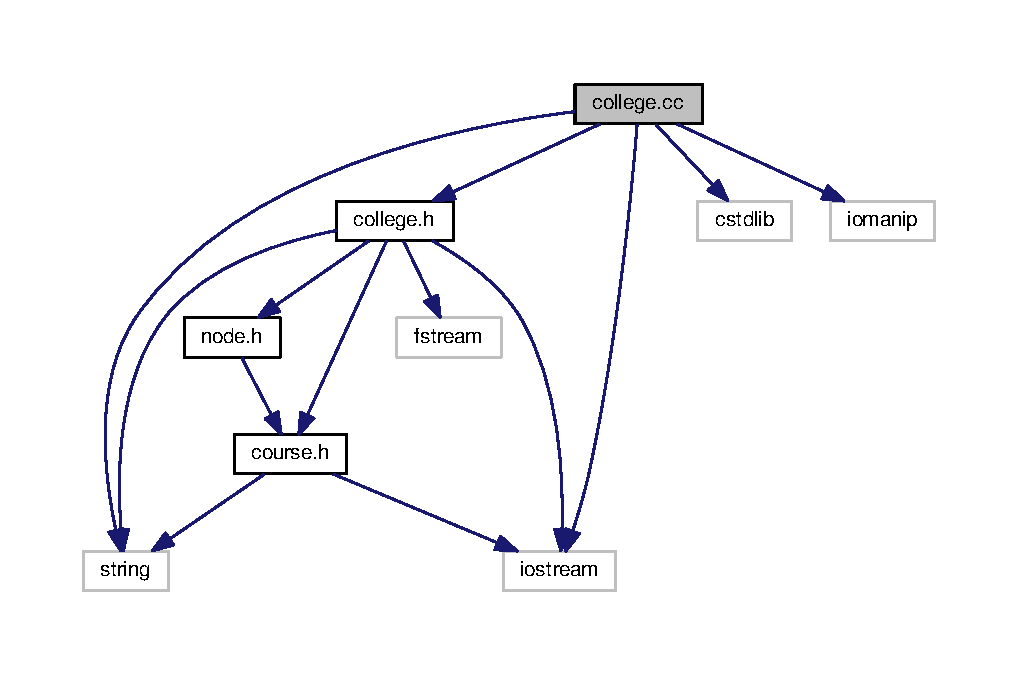
\includegraphics[width=350pt]{college_8cc__incl}
\end{center}
\end{figure}


\subsection{Detailed Description}
This is a linked list to store college data. 

\begin{DoxyAuthor}{Author}
Matthew Aberegg 
\end{DoxyAuthor}

\hypertarget{college_8h}{}\section{college.\+h File Reference}
\label{college_8h}\index{college.\+h@{college.\+h}}


This is the header file for the object college.  


{\ttfamily \#include $<$iostream$>$}\\*
{\ttfamily \#include $<$fstream$>$}\\*
{\ttfamily \#include $<$string$>$}\\*
{\ttfamily \#include \char`\"{}course.\+h\char`\"{}}\\*
{\ttfamily \#include \char`\"{}node.\+h\char`\"{}}\\*
Include dependency graph for college.\+h\+:
\nopagebreak
\begin{figure}[H]
\begin{center}
\leavevmode
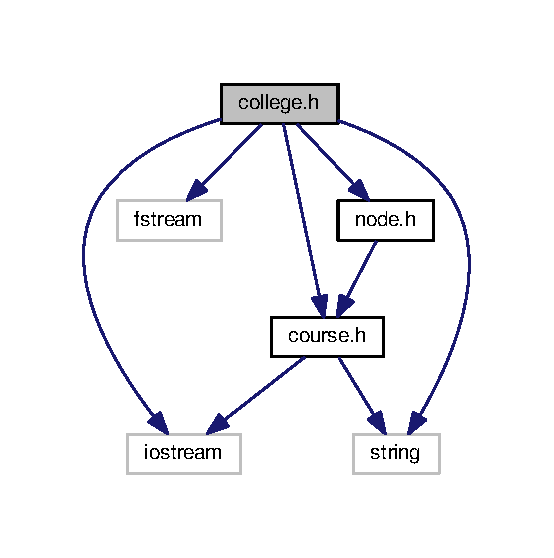
\includegraphics[width=266pt]{college_8h__incl}
\end{center}
\end{figure}
This graph shows which files directly or indirectly include this file\+:
\nopagebreak
\begin{figure}[H]
\begin{center}
\leavevmode
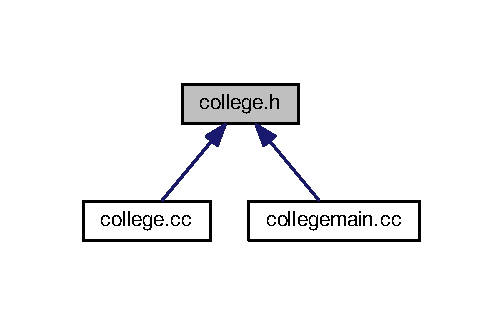
\includegraphics[width=242pt]{college_8h__dep__incl}
\end{center}
\end{figure}
\subsection*{Classes}
\begin{DoxyCompactItemize}
\item 
class \hyperlink{classCollege}{College}
\end{DoxyCompactItemize}


\subsection{Detailed Description}
This is the header file for the object college. 

\begin{DoxyAuthor}{Author}
Matthew Aberegg 
\end{DoxyAuthor}

\hypertarget{collegemain_8cc}{}\section{collegemain.\+cc File Reference}
\label{collegemain_8cc}\index{collegemain.\+cc@{collegemain.\+cc}}


This is the main driver for this project.  


{\ttfamily \#include $<$iostream$>$}\\*
{\ttfamily \#include $<$fstream$>$}\\*
{\ttfamily \#include $<$string$>$}\\*
{\ttfamily \#include \char`\"{}course.\+h\char`\"{}}\\*
{\ttfamily \#include \char`\"{}node.\+h\char`\"{}}\\*
{\ttfamily \#include \char`\"{}college.\+h\char`\"{}}\\*
Include dependency graph for collegemain.\+cc\+:
\nopagebreak
\begin{figure}[H]
\begin{center}
\leavevmode
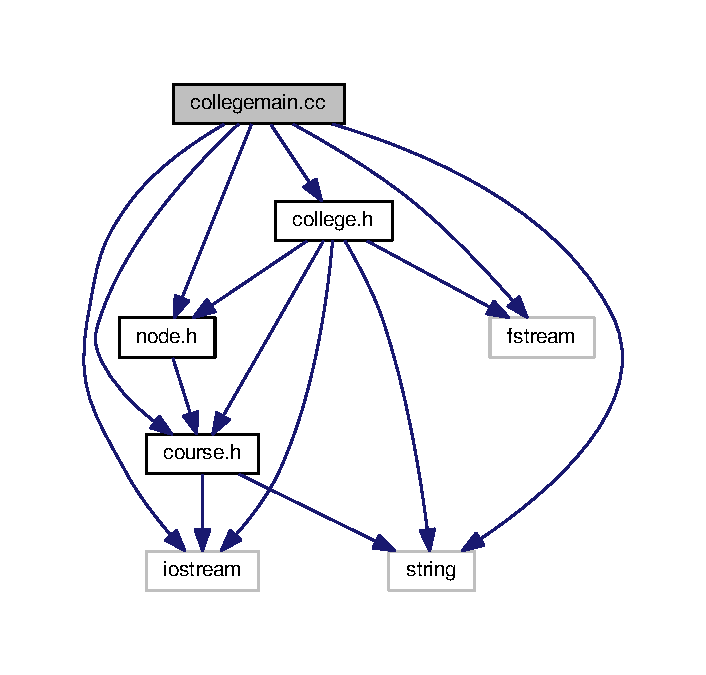
\includegraphics[width=339pt]{collegemain_8cc__incl}
\end{center}
\end{figure}
\subsection*{Functions}
\begin{DoxyCompactItemize}
\item 
int {\bfseries menu} ()\hypertarget{collegemain_8cc_ae83fcdbeb2b6757fc741ae953b633ee1}{}\label{collegemain_8cc_ae83fcdbeb2b6757fc741ae953b633ee1}

\item 
int {\bfseries main} ()\hypertarget{collegemain_8cc_ae66f6b31b5ad750f1fe042a706a4e3d4}{}\label{collegemain_8cc_ae66f6b31b5ad750f1fe042a706a4e3d4}

\end{DoxyCompactItemize}


\subsection{Detailed Description}
This is the main driver for this project. 

\begin{DoxyAuthor}{Author}
John Dolan 
\end{DoxyAuthor}

\hypertarget{course_8cc}{}\section{course.\+cc File Reference}
\label{course_8cc}\index{course.\+cc@{course.\+cc}}


This is the object to describe courses.  


{\ttfamily \#include \char`\"{}course.\+h\char`\"{}}\\*
{\ttfamily \#include $<$cstdlib$>$}\\*
{\ttfamily \#include $<$iostream$>$}\\*
{\ttfamily \#include $<$iomanip$>$}\\*
{\ttfamily \#include $<$string$>$}\\*
Include dependency graph for course.\+cc\+:
\nopagebreak
\begin{figure}[H]
\begin{center}
\leavevmode
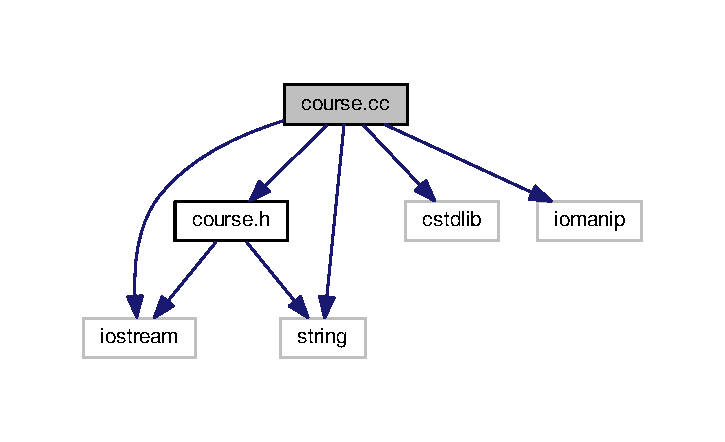
\includegraphics[width=348pt]{course_8cc__incl}
\end{center}
\end{figure}
\subsection*{Functions}
\begin{DoxyCompactItemize}
\item 
istream \& {\bfseries operator$>$$>$} (istream \&ins, \hyperlink{classcourse}{course} \&c)\hypertarget{course_8cc_a2ec0dc87af68602f1724c98787b1234a}{}\label{course_8cc_a2ec0dc87af68602f1724c98787b1234a}

\item 
ostream \& {\bfseries operator$<$$<$} (ostream \&outs, const \hyperlink{classcourse}{course} \&c)\hypertarget{course_8cc_a2530386884877660a5fa7cff8ac917a3}{}\label{course_8cc_a2530386884877660a5fa7cff8ac917a3}

\end{DoxyCompactItemize}


\subsection{Detailed Description}
This is the object to describe courses. 

\begin{DoxyAuthor}{Author}
John Dolan 
\end{DoxyAuthor}

\hypertarget{course_8h}{}\section{course.\+h File Reference}
\label{course_8h}\index{course.\+h@{course.\+h}}


This is the header file for the course object.  


{\ttfamily \#include $<$iostream$>$}\\*
{\ttfamily \#include $<$string$>$}\\*
Include dependency graph for course.\+h\+:
\nopagebreak
\begin{figure}[H]
\begin{center}
\leavevmode
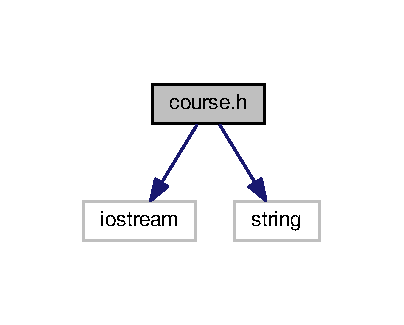
\includegraphics[width=194pt]{course_8h__incl}
\end{center}
\end{figure}
This graph shows which files directly or indirectly include this file\+:
\nopagebreak
\begin{figure}[H]
\begin{center}
\leavevmode
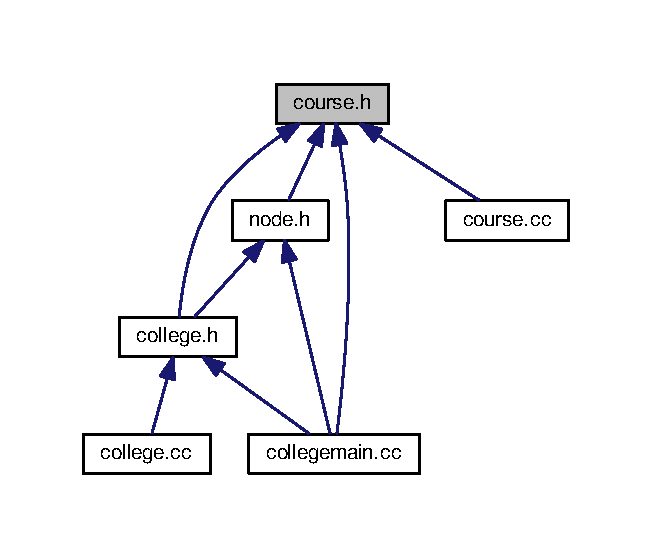
\includegraphics[width=313pt]{course_8h__dep__incl}
\end{center}
\end{figure}
\subsection*{Classes}
\begin{DoxyCompactItemize}
\item 
class \hyperlink{classcourse}{course}
\end{DoxyCompactItemize}
\subsection*{Functions}
\begin{DoxyCompactItemize}
\item 
std\+::istream \& {\bfseries operator$>$$>$} (std\+::istream \&ins, \hyperlink{classcourse}{course} \&c)\hypertarget{course_8h_a65484b76ab377391c8a2b243506e3861}{}\label{course_8h_a65484b76ab377391c8a2b243506e3861}

\item 
std\+::ostream \& {\bfseries operator$<$$<$} (std\+::ostream \&outs, const \hyperlink{classcourse}{course} \&c)\hypertarget{course_8h_a00715c2d2864b3b73aa70eebb700886e}{}\label{course_8h_a00715c2d2864b3b73aa70eebb700886e}

\end{DoxyCompactItemize}


\subsection{Detailed Description}
This is the header file for the course object. 

\begin{DoxyAuthor}{Author}
John Dolan 
\end{DoxyAuthor}

\hypertarget{node_8h}{}\section{node.\+h File Reference}
\label{node_8h}\index{node.\+h@{node.\+h}}


This is a node class to use with linked lists.  


{\ttfamily \#include \char`\"{}course.\+h\char`\"{}}\\*
Include dependency graph for node.\+h\+:
\nopagebreak
\begin{figure}[H]
\begin{center}
\leavevmode
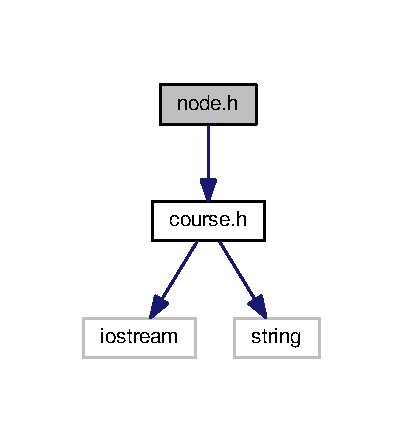
\includegraphics[width=194pt]{node_8h__incl}
\end{center}
\end{figure}
This graph shows which files directly or indirectly include this file\+:
\nopagebreak
\begin{figure}[H]
\begin{center}
\leavevmode
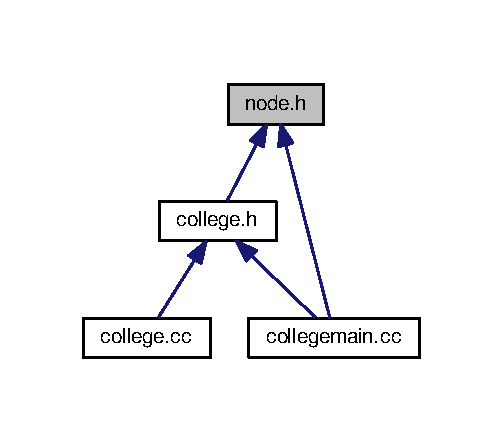
\includegraphics[width=242pt]{node_8h__dep__incl}
\end{center}
\end{figure}
\subsection*{Classes}
\begin{DoxyCompactItemize}
\item 
class \hyperlink{classnode}{node}
\end{DoxyCompactItemize}


\subsection{Detailed Description}
This is a node class to use with linked lists. 

\begin{DoxyAuthor}{Author}
John Dolan 
\end{DoxyAuthor}

\hypertarget{tarray_8h}{}\section{tarray.\+h File Reference}
\label{tarray_8h}\index{tarray.\+h@{tarray.\+h}}


This file is used in understanding template arrays.  


{\ttfamily \#include $<$iostream$>$}\\*
{\ttfamily \#include \char`\"{}tarray.\+template\char`\"{}}\\*
Include dependency graph for tarray.\+h\+:
\nopagebreak
\begin{figure}[H]
\begin{center}
\leavevmode
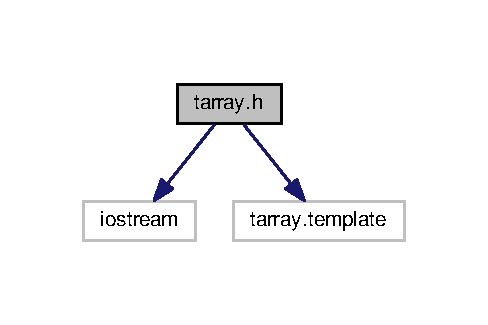
\includegraphics[width=234pt]{tarray_8h__incl}
\end{center}
\end{figure}
\subsection*{Classes}
\begin{DoxyCompactItemize}
\item 
class \hyperlink{classTarray}{Tarray$<$ T $>$}
\end{DoxyCompactItemize}


\subsection{Detailed Description}
This file is used in understanding template arrays. 

\begin{DoxyAuthor}{Author}
John Dolan 
\end{DoxyAuthor}

%--- End generated contents ---

% Index
\backmatter
\newpage
\phantomsection
\clearemptydoublepage
\addcontentsline{toc}{chapter}{Index}
\printindex

\end{document}
